\documentclass[14pt]{extbook}
\usepackage{multicol, enumerate, enumitem, hyperref, color, soul, setspace, parskip, fancyhdr} %General Packages
\usepackage{amssymb, amsthm, amsmath, latexsym, units, mathtools} %Math Packages
\everymath{\displaystyle} %All math in Display Style
% Packages with additional options
\usepackage[headsep=0.5cm,headheight=12pt, left=1 in,right= 1 in,top= 1 in,bottom= 1 in]{geometry}
\usepackage[usenames,dvipsnames]{xcolor}
\usepackage{dashrule}  % Package to use the command below to create lines between items
\newcommand{\litem}[1]{\item#1\hspace*{-1cm}\rule{\textwidth}{0.4pt}}
\pagestyle{fancy}
\lhead{Makeup Progress Quiz 2}
\chead{}
\rhead{Version B}
\lfoot{5763-3522}
\cfoot{}
\rfoot{Spring 2021}
\begin{document}

\begin{enumerate}
\litem{
Construct the lowest-degree polynomial given the zeros below. Then, choose the intervals that contain the coefficients of the polynomial in the form $ax^3+bx^2+cx+d$.\[ \frac{1}{3}, 7, \text{ and } \frac{5}{3} \]\begin{enumerate}[label=\Alph*.]
\item \( a \in [2, 13], b \in [-83, -77], c \in [129, 133], \text{ and } d \in [-38, -33] \)
\item \( a \in [2, 13], b \in [-83, -77], c \in [129, 133], \text{ and } d \in [35, 38] \)
\item \( a \in [2, 13], b \in [79, 93], c \in [129, 133], \text{ and } d \in [35, 38] \)
\item \( a \in [2, 13], b \in [-77, -74], c \in [79, 80], \text{ and } d \in [35, 38] \)
\item \( a \in [2, 13], b \in [51, 52], c \in [-90, -84], \text{ and } d \in [-38, -33] \)

\end{enumerate} }
\litem{
Construct the lowest-degree polynomial given the zeros below. Then, choose the intervals that contain the coefficients of the polynomial in the form $x^3+bx^2+cx+d$.\[ 4 - 5 i \text{ and } 1 \]\begin{enumerate}[label=\Alph*.]
\item \( b \in [1, 3], c \in [-11, -4], \text{ and } d \in [2, 9] \)
\item \( b \in [5, 20], c \in [49, 51], \text{ and } d \in [38, 46] \)
\item \( b \in [1, 3], c \in [0, 9], \text{ and } d \in [-11, 2] \)
\item \( b \in [-17, -5], c \in [49, 51], \text{ and } d \in [-44, -38] \)
\item \( \text{None of the above.} \)

\end{enumerate} }
\litem{
Which of the following equations \textit{could} be of the graph presented below?
\begin{center}
    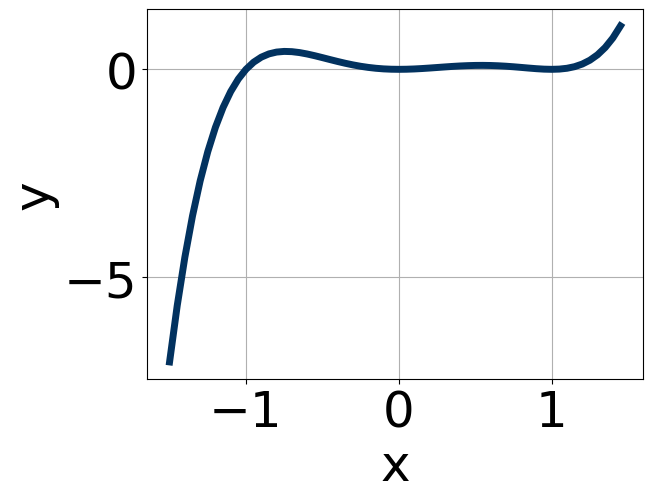
\includegraphics[width=0.5\textwidth]{../Figures/polyGraphToFunctionB.png}
\end{center}
\begin{enumerate}[label=\Alph*.]
\item \( 9x^{9} (x - 1)^{8} (x + 1)^{11} \)
\item \( -9x^{8} (x - 1)^{8} (x + 1)^{7} \)
\item \( -20x^{8} (x - 1)^{4} (x + 1)^{4} \)
\item \( 8x^{9} (x - 1)^{8} (x + 1)^{6} \)
\item \( 8x^{4} (x - 1)^{4} (x + 1)^{5} \)

\end{enumerate} }
\litem{
Describe the zero behavior of the zero $x = -4$ of the polynomial below.\[ f(x) = 8(x + 4)^{9}(x - 4)^{12}(x - 7)^{5}(x + 7)^{9} \]\begin{enumerate}[label=\Alph*.]
\begin{multicols}{2}\item 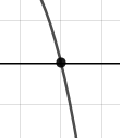
\includegraphics[width = 0.3\textwidth]{../Figures/polyZeroBehaviorCopyAB.png}\item 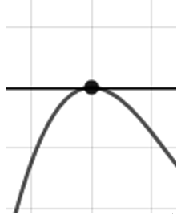
\includegraphics[width = 0.3\textwidth]{../Figures/polyZeroBehaviorCopyBB.png}\item 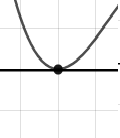
\includegraphics[width = 0.3\textwidth]{../Figures/polyZeroBehaviorCopyCB.png}\item 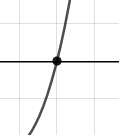
\includegraphics[width = 0.3\textwidth]{../Figures/polyZeroBehaviorCopyDB.png}\end{multicols}\item None of the above.
\end{enumerate} }
\litem{
Describe the zero behavior of the zero $x = -8$ of the polynomial below.\[ f(x) = 3(x + 6)^{6}(x - 6)^{2}(x - 8)^{9}(x + 8)^{6} \]\begin{enumerate}[label=\Alph*.]
\begin{multicols}{2}\item 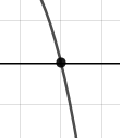
\includegraphics[width = 0.3\textwidth]{../Figures/polyZeroBehaviorAB.png}\item 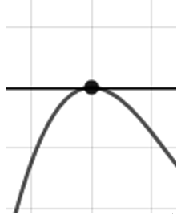
\includegraphics[width = 0.3\textwidth]{../Figures/polyZeroBehaviorBB.png}\item 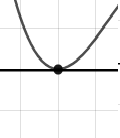
\includegraphics[width = 0.3\textwidth]{../Figures/polyZeroBehaviorCB.png}\item 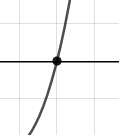
\includegraphics[width = 0.3\textwidth]{../Figures/polyZeroBehaviorDB.png}\end{multicols}\item None of the above.
\end{enumerate} }
\litem{
Construct the lowest-degree polynomial given the zeros below. Then, choose the intervals that contain the coefficients of the polynomial in the form $x^3+bx^2+cx+d$.\[ -5 + 5 i \text{ and } 2 \]\begin{enumerate}[label=\Alph*.]
\item \( b \in [-5, 6], c \in [-9, 1], \text{ and } d \in [7, 22] \)
\item \( b \in [-12, -2], c \in [29, 38], \text{ and } d \in [92, 102] \)
\item \( b \in [6, 14], c \in [29, 38], \text{ and } d \in [-106, -99] \)
\item \( b \in [-5, 6], c \in [-1, 4], \text{ and } d \in [-21, -9] \)
\item \( \text{None of the above.} \)

\end{enumerate} }
\litem{
Construct the lowest-degree polynomial given the zeros below. Then, choose the intervals that contain the coefficients of the polynomial in the form $ax^3+bx^2+cx+d$.\[ \frac{1}{4}, 7, \text{ and } \frac{-7}{5} \]\begin{enumerate}[label=\Alph*.]
\item \( a \in [20, 22], b \in [-122, -116], c \in [-170, -163], \text{ and } d \in [46, 52] \)
\item \( a \in [20, 22], b \in [165, 181], c \in [238, 243], \text{ and } d \in [46, 52] \)
\item \( a \in [20, 22], b \in [-109, -104], c \in [-227, -217], \text{ and } d \in [-53, -44] \)
\item \( a \in [20, 22], b \in [114, 125], c \in [-170, -163], \text{ and } d \in [-53, -44] \)
\item \( a \in [20, 22], b \in [-122, -116], c \in [-170, -163], \text{ and } d \in [-53, -44] \)

\end{enumerate} }
\litem{
Describe the end behavior of the polynomial below.\[ f(x) = 7(x + 4)^{3}(x - 4)^{8}(x - 5)^{4}(x + 5)^{4} \]\begin{enumerate}[label=\Alph*.]
\begin{multicols}{2}\item 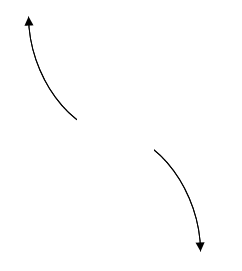
\includegraphics[width = 0.3\textwidth]{../Figures/polyEndBehaviorCopyAB.png}\item 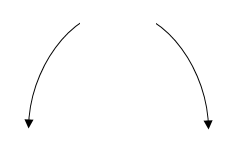
\includegraphics[width = 0.3\textwidth]{../Figures/polyEndBehaviorCopyBB.png}\item 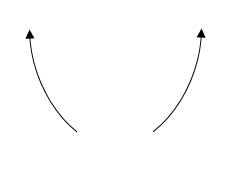
\includegraphics[width = 0.3\textwidth]{../Figures/polyEndBehaviorCopyCB.png}\item 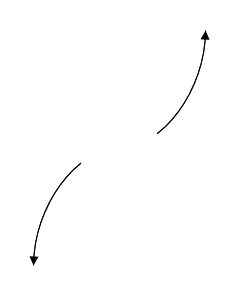
\includegraphics[width = 0.3\textwidth]{../Figures/polyEndBehaviorCopyDB.png}\end{multicols}\item None of the above.
\end{enumerate} }
\litem{
Which of the following equations \textit{could} be of the graph presented below?
\begin{center}
    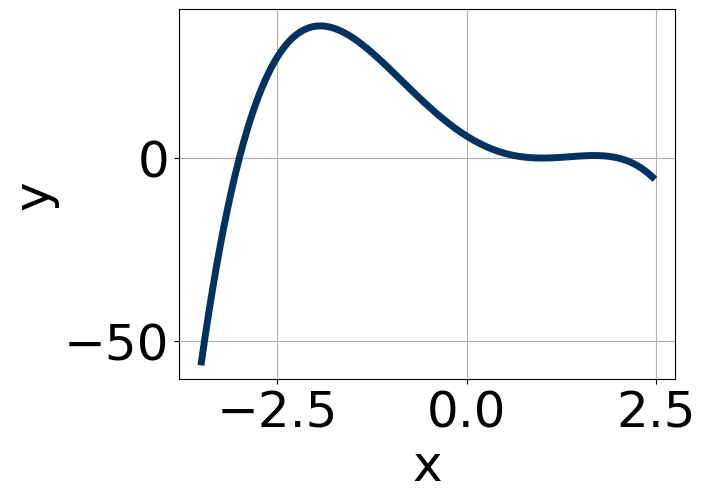
\includegraphics[width=0.5\textwidth]{../Figures/polyGraphToFunctionCopyB.png}
\end{center}
\begin{enumerate}[label=\Alph*.]
\item \( -5(x - 1)^{10} (x + 3)^{6} (x - 2)^{9} \)
\item \( 3(x - 1)^{10} (x + 3)^{9} (x - 2)^{6} \)
\item \( -3(x - 1)^{11} (x + 3)^{6} (x - 2)^{9} \)
\item \( 18(x - 1)^{6} (x + 3)^{9} (x - 2)^{5} \)
\item \( -4(x - 1)^{4} (x + 3)^{5} (x - 2)^{9} \)

\end{enumerate} }
\litem{
Describe the end behavior of the polynomial below.\[ f(x) = 9(x - 6)^{2}(x + 6)^{3}(x + 8)^{5}(x - 8)^{7} \]\begin{enumerate}[label=\Alph*.]
\begin{multicols}{2}\item 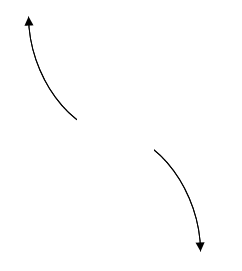
\includegraphics[width = 0.3\textwidth]{../Figures/polyEndBehaviorAB.png}\item 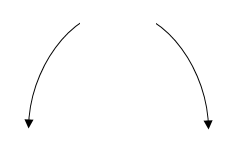
\includegraphics[width = 0.3\textwidth]{../Figures/polyEndBehaviorBB.png}\item 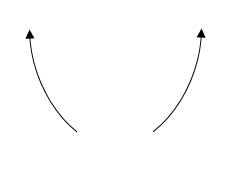
\includegraphics[width = 0.3\textwidth]{../Figures/polyEndBehaviorCB.png}\item 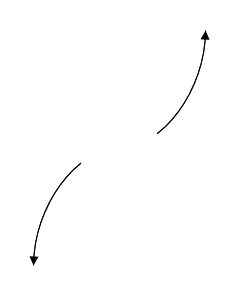
\includegraphics[width = 0.3\textwidth]{../Figures/polyEndBehaviorDB.png}\end{multicols}\item None of the above.
\end{enumerate} }
\end{enumerate}

\end{document}